\section{5Guard Baseline}\label{sec:fiveguard}
To address this trade-off, the baseline framework \textit{5Guard: Isolation-Aware End-to-End Slicing of 5G Networks} was proposed~\cite{bolourian2026fiveguard}. 5Guard explicitly defines three isolation levels: Level 0 (L0) for logical sharing, Level 1 (L1) for virtual isolation via hypervisors, and Level 2 (L2) for complete physical isolation (e.g., dedicated CPU cores and radio guardbands). 

The authors formulate the resource allocation problem as a massive Mixed-Integer Linear Program (MILP) that optimizes slice placement across the RAN, Transport, and Core domains to maximize InP profit. The mathematical model rigorously accounts for the cost of deploying Virtual Network Functions (VNFs), the penalty of isolation overheads (such as reserving dedicated CPU pinning for L2), and the cost of bandwidth on the transport links. 

Because solving this MILP is NP-Hard and computationally prohibitive for large networks, 5Guard utilizes an ensemble of algorithms to find near-optimal placements under strict time deadlines. This ensemble includes the exact mathematical solver (OPT) which guarantees optimal profit but is slow, alongside rapid heuristic fallback algorithms like Isolation-Aware Routing (IAR) and Delay-Tolerant Routing (DTR) that rely on graph-traversal to quickly embed slices before their admission timeout expires.

\subsection{End-to-End 5G Slicing Model}
Figure~\ref{fig:basepaper-system-model} shows the end-to-end system model used by 5Guard. A slice spans the Radio Access Network (RAN), the transport network, and the 5G Core (5GC). Its radio units, distributed units, centralized units, and core network functions must be mapped onto physical radio, optical, and computing resources. The diagram also illustrates that isolation is an end-to-end property: assigning a high isolation level affects resources in every domain rather than only the virtual machines hosting the network functions.

\begin{figure}[htbp]
\centering
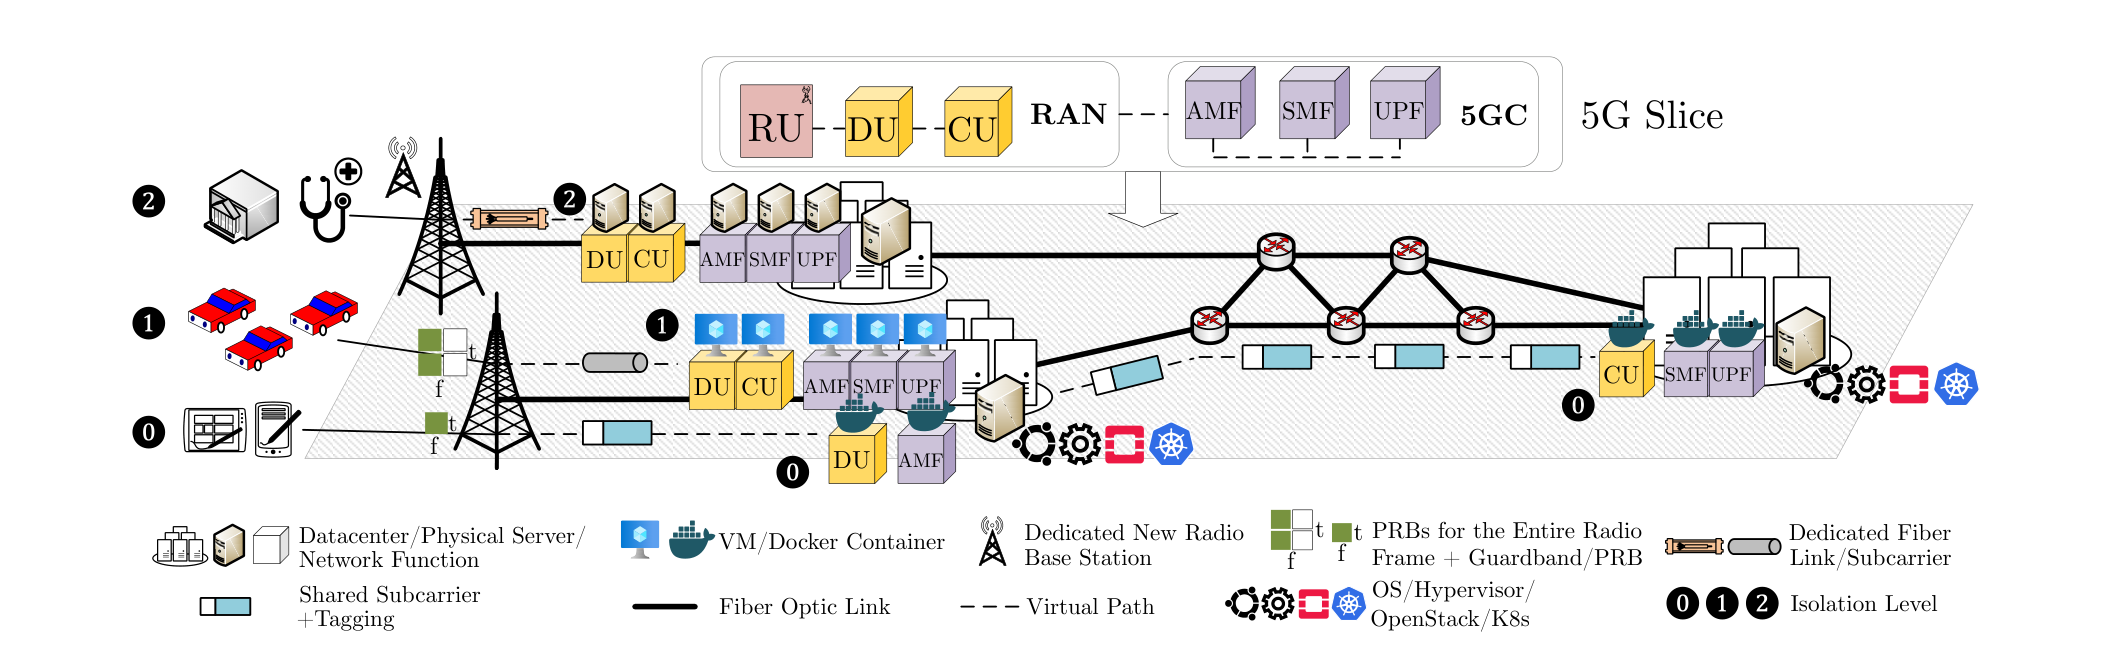
\includegraphics[width=\textwidth]{basepaper_system_model.png}
\caption[5Guard end-to-end slicing system model]{End-to-end isolation-aware 5G slicing system model. Reproduced from Fig.~1 of the 5Guard base paper~\cite{bolourian2026fiveguard}.}
\label{fig:basepaper-system-model}
\end{figure}

The three example service classes on the left of Figure~\ref{fig:basepaper-system-model} demonstrate the intended use of the levels. Critical services receive complete isolation, vehicular services receive semi-isolation, and best-effort services use shared resources. This distinction is central to SecGuard because the proposed risk engine changes the isolation input supplied to the allocator when observed traffic risk increases.

\subsection{Isolation Levels and Resource Overheads}
Figure~\ref{fig:basepaper-isolation-levels} explains how the three isolation levels are realized across the radio, transport, and MEC/cloud domains. At Level 0, slices share radio blocks, transport capacity, and containerized computing resources. Level 1 introduces stronger logical separation through radio guard bands, dedicated wavelength portions, virtual machines, hypervisors, and operating-system overhead. Level 2 reserves physical infrastructure, such as a dedicated base station, fiber resource, or physical server.

\begin{figure}[htbp]
\centering
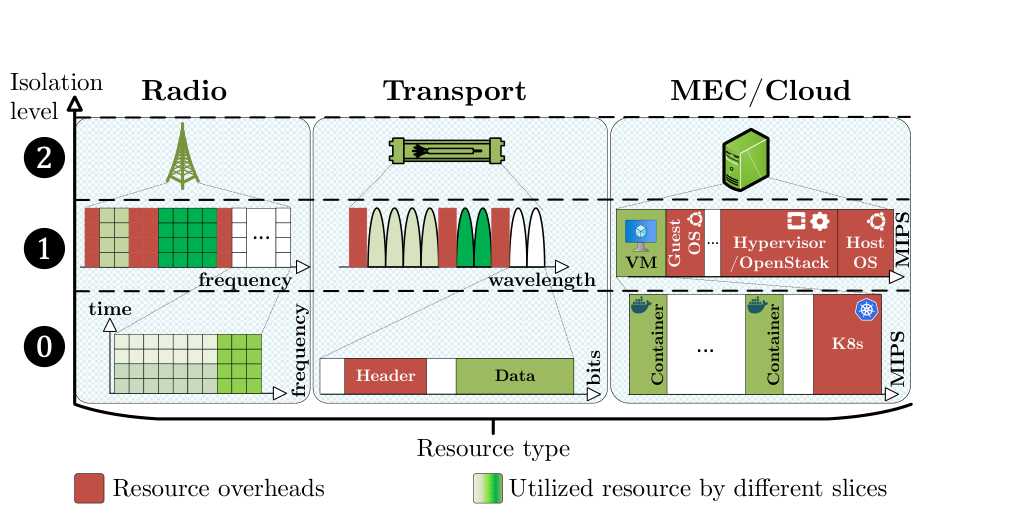
\includegraphics[width=0.72\textwidth]{basepaper_isolation_levels.png}
\caption[5Guard isolation levels and resource overheads]{Isolation levels and their resource overheads in the radio, transport, and MEC/cloud domains. Reproduced from Fig.~2 of the 5Guard base paper~\cite{bolourian2026fiveguard}.}
\label{fig:basepaper-isolation-levels}
\end{figure}

The red portions in Figure~\ref{fig:basepaper-isolation-levels} represent overhead introduced by isolation mechanisms. Stronger isolation can therefore improve separation while consuming capacity that could otherwise admit additional slices. This security--resource trade-off motivates SecGuard's use of risk-dependent upgrades instead of assigning the strongest isolation level to every slice.

Table~\ref{tab:isolation-summary} summarizes the isolation mechanisms illustrated in the base paper and the corresponding resource trade-offs.
\begin{table}[htbp]
\centering\small
\caption[Isolation mechanisms across network domains]{Isolation mechanisms across network domains, summarized from 5Guard~\cite{bolourian2026fiveguard}}
\label{tab:isolation-summary}
\renewcommand{\arraystretch}{1.2}
\begin{tabularx}{\textwidth}{|p{0.08\textwidth}|Y|Y|Y|}
\hline
\textbf{Level} & \textbf{Radio} & \textbf{Transport} & \textbf{MEC/cloud} \\
\hline
L0 & Shared base station with scheduled radio blocks & Shared subcarriers with tagging & Containerized functions on shared computing infrastructure \\
\hline
L1 & Radio blocks reserved across a frame with guard bands & Dedicated subcarriers and guard bands & Virtual machines with guest OS and hypervisor overhead \\
\hline
L2 & Dedicated base station & Dedicated fiber resource & Dedicated physical server \\
\hline
\end{tabularx}
\end{table}

\subsection{5Guard Ensemble Workflow}
Figure~\ref{fig:basepaper-flow} presents the 5Guard decision process. OPT, RNR, DTR, and IAR receive the same network state and slice request and run concurrently. Each algorithm offers a different balance between execution time and profit. When the allocation deadline is reached, unfinished executions are stopped and the framework selects the most profitable feasible solution returned within the deadline.

\begin{figure}[htbp]
\centering
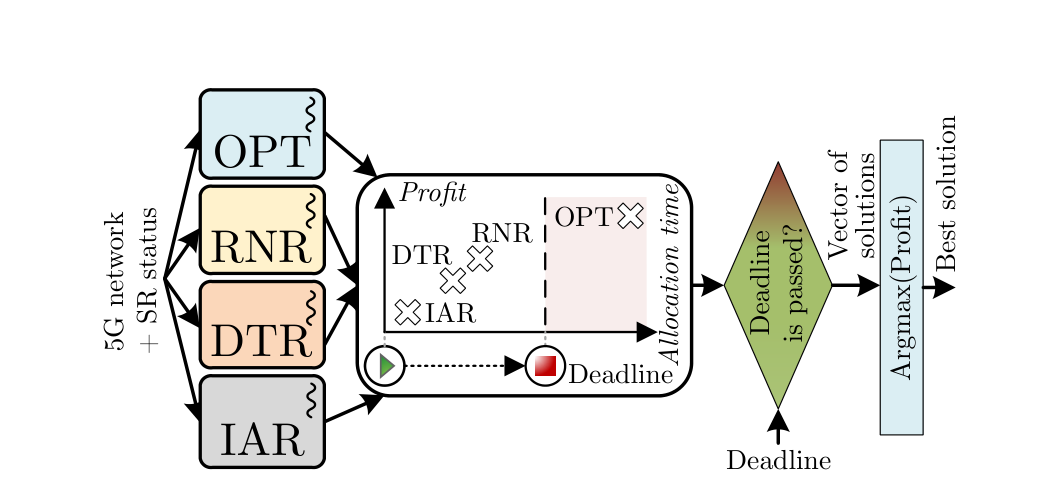
\includegraphics[width=0.68\textwidth]{basepaper_5guard_flow.png}
\caption[5Guard ensemble workflow]{Flow of the 5Guard optimization ensemble and deadline-based solution selection. Reproduced from Fig.~3 of the 5Guard base paper~\cite{bolourian2026fiveguard}.}
\label{fig:basepaper-flow}
\end{figure}

This workflow provides the allocation foundation used by SecGuard. The current contribution changes the isolation requirement presented to the allocator; it does not replace 5Guard's resource-placement formulation. The planned algorithm-selection objective would later use request and network features to avoid running unsuitable ensemble members when their expected computation cost is too high.

\section{Related Methods and Research Gap}\label{sec:gap}
The 5Guard formulation connects requested isolation levels to end-to-end resource placement, but the request is fixed at admission. SecGuard studies a separate control question: how traffic-derived risk can change the isolation input while retaining the tenant's minimum requested level. Random forests provide the classifier used for traffic risk estimation~\cite{breiman2001random}; the 5G intrusion dataset supplies the flow records used in the preliminary detector experiment~\cite{open5gsdataset}. The work reported here integrates these components with a 5Guard-style allocator. It does not establish prevention of cross-slice attack propagation.

Prior work has examined isolation-aware resource allocation and service orchestration in 5G slicing~\cite{su2019isolation,taleb2019industrial}. SecGuard builds on this line of work by connecting a traffic-derived risk signal to the isolation request passed to the allocator.

\section{Research Questions}\label{sec:research-questions}
This report asks whether a traffic-risk policy can preserve the requested isolation floor while reducing a modeled exposure measure, how much profit is recovered relative to a fixed security policy, and what remains to be tested before admission control and algorithm selection can be evaluated.
